% Asset ID: A21TrigonometryAndModellingTikZ-003
% Purpose: Double angle formula tree
\documentclass[tikz,border=10pt]{standalone}
\usepackage{amsmath}
\usetikzlibrary{arrows.meta,positioning}
\begin{document}
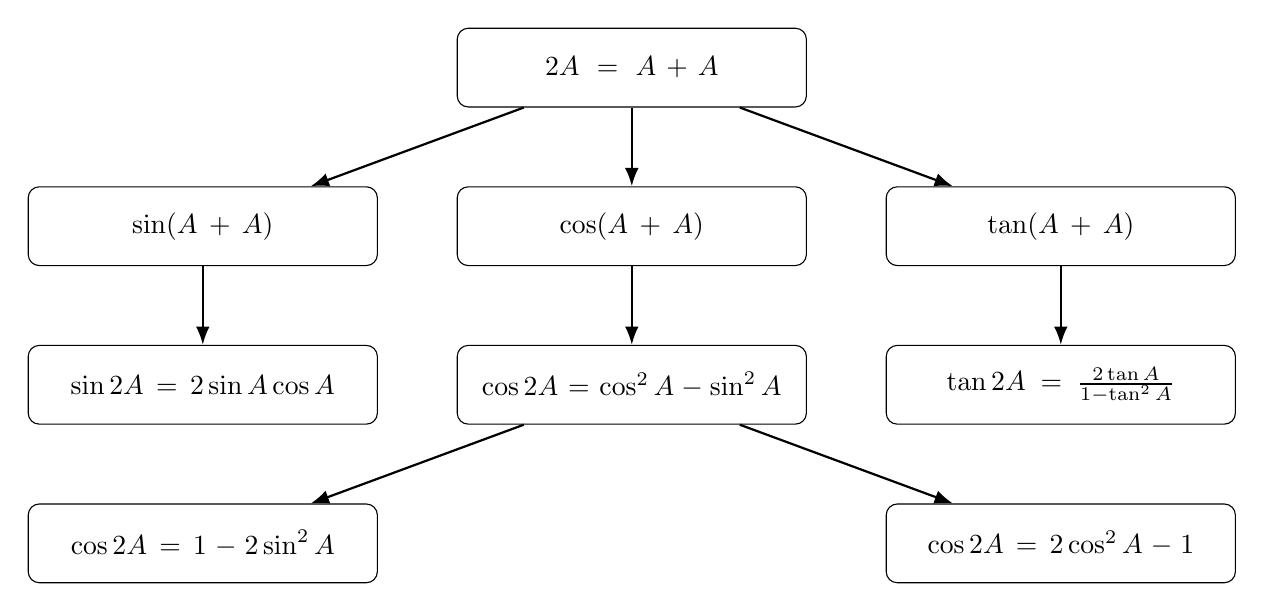
\begin{tikzpicture}[node distance=1cm and 1cm,box/.style={draw,rounded corners,align=center,text width=4.2cm,minimum height=1cm},arrow/.style={-Latex,thick}]
\node[box,font=\bfseries] (start) {\(2A=A+A\)};
\node[box,below left=of start] (sin) {\(\sin(A+A)\)};
\node[box,below=of start] (cos) {\(\cos(A+A)\)};
\node[box,below right=of start] (tan) {\(\tan(A+A)\)};
\node[box,below=of sin] (sinr) {\(\sin2A=2\sin A\cos A\)};
\node[box,below=of cos] (cosr) {\(\cos2A=\cos^2A-\sin^2A\)};
\node[box,below=of tan] (tanr) {\(\tan2A=\frac{2\tan A}{1-\tan^2A}\)};
\node[box,below left=of cosr] (c1) {\(\cos2A=1-2\sin^2A\)};
\node[box,below right=of cosr] (c2) {\(\cos2A=2\cos^2A-1\)};
\draw[arrow] (start)--(sin); \draw[arrow] (start)--(cos); \draw[arrow] (start)--(tan);
\draw[arrow] (sin)--(sinr); \draw[arrow] (cos)--(cosr); \draw[arrow] (tan)--(tanr);
\draw[arrow] (cosr)--(c1); \draw[arrow] (cosr)--(c2);
\end{tikzpicture}
\end{document}
